\documentclass[UTF8,11pt,a4paper]{ctexart}
\newcommand{\DocTitle}{项目实施方案}
\newcommand{\DocSubtitle}{基线、模块契约和验收}
% Shared layout for the CW2 companion documents.
\usepackage[margin=2.1cm,headheight=16pt]{geometry}
\usepackage{amsmath,amssymb,booktabs,array,tabularx,ragged2e}
\usepackage{enumitem,xcolor,fancyhdr,listings,tcolorbox}
\tcbuselibrary{breakable}
\usepackage{hyperref}
\usepackage{bookmark}

\newcommand{\DocVersion}{3.0}
\newcommand{\EngineVersion}{1.1}
\newcommand{\DocDate}{2026-11-23}
\definecolor{ink}{HTML}{1F2937}
\definecolor{accent}{HTML}{92400E}
\definecolor{muted}{HTML}{4B5563}
\definecolor{linkink}{HTML}{174678}
\definecolor{codebg}{HTML}{F5F7FA}
\hypersetup{unicode,colorlinks=true,linkcolor=linkink,urlcolor=linkink,
  filecolor=linkink,pdftitle={SOE104 CW2 \DocTitle\space v\DocVersion},
  pdfauthor={Group A--E}}
\ctexset{section={format={\Large\bfseries\color{accent}}},
  subsection={format={\large\bfseries\color{ink}}}}
\pagestyle{fancy}
\fancyhf{}
\fancyhead[L]{\small\color{muted}SOE104 CW2 · Oregon Trail}
\fancyhead[R]{\small\color{muted}\DocTitle\ v\DocVersion}
\fancyfoot[C]{\small\color{muted}\thepage}
\renewcommand{\headrulewidth}{0.4pt}
\setlength{\parskip}{0.35em}
\setlength{\emergencystretch}{1.5em}
\renewcommand{\arraystretch}{1.23}
\setlist{itemsep=3pt,topsep=3pt,parsep=0pt,leftmargin=1.7em}
\newcolumntype{Y}{>{\RaggedRight\arraybackslash}X}
\newcolumntype{L}[1]{>{\RaggedRight\arraybackslash}p{#1}}
\newtcolorbox{keybox}[1]{breakable,title={#1},colback=orange!4,
  colframe=accent,boxrule=0.55pt,arc=2pt,fonttitle=\bfseries}
\newtcolorbox{warnbox}[1]{breakable,title={#1},colback=red!3,
  colframe=red!45!black,boxrule=0.55pt,arc=2pt,fonttitle=\bfseries}
\lstset{basicstyle=\small\ttfamily,backgroundcolor=\color{codebg},
  xleftmargin=0.9em,frame=l,rulecolor=\color{linkink!45},
  breaklines=true,columns=fullflexible,keepspaces=true,showstringspaces=false,
  aboveskip=0.65em,belowskip=0.65em}
\newcommand{\code}[1]{\texttt{#1}}
\newcommand{\source}[1]{\textup{\small\textcolor{muted}{[#1]}}}
\newcommand{\docref}[2]{\href{./#1.pdf}{#2}}
\renewcommand{\maketitle}{%
  \begin{center}
    {\LARGE\bfseries CW2 \DocTitle\par}
    \vspace{0.35em}{\large\DocSubtitle\par}
    \vspace{0.75em}{\small\color{muted}Group A--E · 整理：A
      \quad\DocDate\quad 文档 v\DocVersion\par}
    \vspace{0.2em}{\small\color{muted}Engine / Marking v\EngineVersion\par}
  \end{center}
  \vspace{0.4em}}

\usepackage{tikz}
\usetikzlibrary{arrows.meta}

\begin{document}
\maketitle
\thispagestyle{fancy}

\begin{keybox}{项目的两个验收层级}
JDK 21 本地编译通过是集成门槛。平台三个种子正常结算并提供回放是运行门槛。
到达率、健康和货物分项用来比较策略。课程提交格式以\docref{02_grading}{《02 评分与提交》}为准。
\end{keybox}

\section{当前基线}

仓库已有 8 个 Java 文件和 \code{lib/oregon-api.jar}。当前由 \code{TeamFactory} 创建
Hunter、Doctor、Mechanic、Scout，采购 4 牛、500 粮、100 弹药、2 零件，余 \$320。
配速固定 \code{NORMAL}，以 \code{MEAGER} 的全车粮食续航 3 回合作为降到
\code{BARE} 的基线阈值。事件处理统一返回 \code{SAFE}。
这些选择为后续对比提供起点。基线描述来自当前源码，平台结果需查实际提交回放。

Hunter 始终狩猎，Doctor 始终治疗，Mechanic 受威胁时防守、其余回合推进，
Scout 负责探路。

\section{模块与数据流}

\noindent\textbf{开局装配。}\code{TeamFactory} 创建成员、策略和事件处理器。
工厂持有一份 \code{Plans}，把同一个对象交给策略和事件处理器。

\begin{center}
\begin{tikzpicture}[
  x=1cm,y=1cm,
  turnnode/.style={rectangle,rounded corners=2pt,draw=linkink!60,
    fill=linkink!5,minimum width=4.4cm,minimum height=1.0cm,align=center,inner sep=4pt},
  flow/.style={-{Latex[length=2.3mm]},draw=linkink,semithick},
  flowlabel/.style={font=\small,text=ink,above=2.5pt}
]
  \node[turnnode] (strategy) at (2.2,0)
    {\code{TeamStrategy}\\{\small\color{muted}回合开始：选配速和口粮}};
  \node[turnnode,draw=accent!65,fill=orange!7,minimum width=2.7cm] (plans) at (8.25,0)
    {\code{Plans}\\{\small\color{muted}保存本轮状态}};
  \node[turnnode] (resolver) at (14.3,0)
    {\code{TeamResolver}\\{\small\color{muted}遇到事件时：选应对方式}};
  \draw[flow] (strategy.east) -- node[flowlabel] {写入状态} (plans.west);
  \draw[flow,dashed] (plans.east) -- node[flowlabel] {提供快照} (resolver.west);
\end{tikzpicture}
\par\smallskip
{\small\color{muted}虚线表示计划接入的快照读取。当前解析器固定返回 \code{SAFE}。}
\end{center}

\noindent\textbf{成员继承。}下面四个成员类分别沿用各自职业的能力，自己实现每回合的动作。

\begin{center}
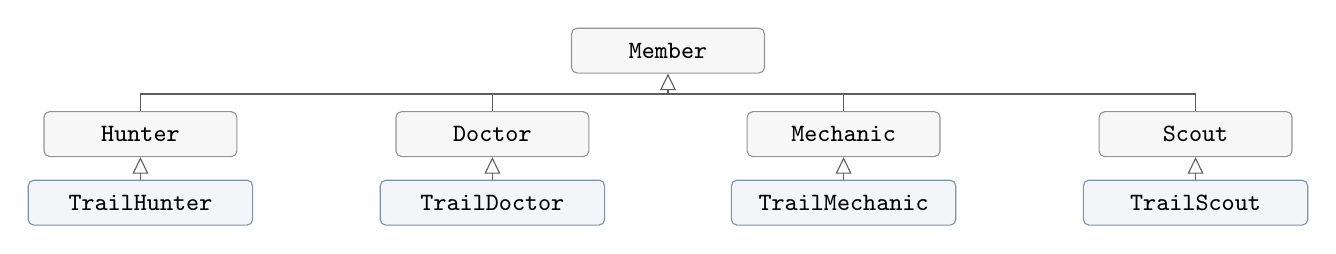
\begin{tikzpicture}[
  x=1cm,y=1cm,
  base/.style={rectangle,rounded corners=2pt,draw=black!42,fill=black!3,
    minimum width=2.45cm,minimum height=0.57cm,font=\small},
  projectrole/.style={base,draw=linkink!58,fill=linkink!5,minimum width=2.85cm},
  inherits/.style={-{Triangle[open,length=2.1mm,width=2.0mm]},draw=black!63}
]
  \node[base] (member) at (8.25,0) {\code{Member}};
  \foreach \x/\job/\file in {
    1.55/Hunter/TrailHunter,6.02/Doctor/TrailDoctor,
    10.48/Mechanic/TrailMechanic,14.95/Scout/TrailScout}{
    \node[base] (\job) at (\x,-1.06) {\code{\job}};
    \node[projectrole] (\file) at (\x,-1.93) {\code{\file}};
    \draw[inherits] (\file.north) -- (\job.south);
    \draw[black!63] (\job.north) -- (\x,-0.55);
  }
  \draw[black!63] (1.55,-0.55) -- (14.95,-0.55);
  \draw[inherits] (8.25,-0.55) -- (member.south);
\end{tikzpicture}
\par\smallskip
{\small\color{muted}空心三角指向父类。成员用引擎传来的 \code{Situation} 决定动作。}
\end{center}

\clearpage
\subsection*{模块接口速查}

\begin{center}\small
\begin{tabularx}{\linewidth}{@{}L{3.8cm}Y@{}}
\toprule
类 & 职责和依赖 \\
\midrule
\code{TeamFactory} & 唯一的 \code{PartyFactory} 实现。组装成员、采购清单、策略与解析器，
将同一个 \code{Plans} 传给策略与解析器。 \\
\code{TeamStrategy} & 实现 \code{PartyStrategy}。读 \code{PartyState}，选定配速和口粮，
发布与本轮指令匹配的快照，再返回 \code{Directive}。 \\
\code{Plans} & 项目自有的共享上下文。设计目标是集中发布带回合号的不可变快照，
同时提供开头状态与事件时预测。 \\
\code{TeamResolver} & 实现 \code{Resolver}。读 \code{Event} 和同回合快照。
普通过程选姿态，市场构造交易或离开，缺快照时按事件类型回退。 \\
四个 \code{Trail} 成员类 & 分别继承对应职业类，重写 \code{act(Situation)}。
结合自身健康和实际收到的 \code{Situation} 决策。 \\
\bottomrule
\end{tabularx}
\end{center}
\noindent
\code{Plans} 的目标契约与伪代码以\docref{04_decision_model}{《04 决策模型》}为准。
成员保持独立，策略与解析器通过快照协调。成员接口未提供全队逐人健康及原生饥饿标志。

\section{把基线改成可测试的策略}

\begin{enumerate}
  \item \textbf{先对齐快照。}把回合初始值与事件时推算值分别标注。
  第 120 回合策略仍有一次当前行进，事件阶段已无未来配速行进。
  若快照缺失或回合不符，返回该事件的兜底选项。
  \item \textbf{再闭合粮食和里程。}检查每档口粮是否足够喂饱成员，另计牛耗粮。
  预测里程包含配速、实际分工能贡献的动作里程与绕道余量。
  失牛后重算运力与可达性。优先修复采购、猎粮和配速之间的矛盾。
  \item \textbf{分批升级事件。}先验证费用、伤害与库存边界，再处理严重度。
  第 04 份文档的基准阈值适用于其设定条件。有致死、断粮或超时风险时按状态重算。
  交易比较挂牌价、议价失败后果和可成交量。
  \item \textbf{在同一组种子上对照。}用上一份可用提交作基线，一次改一类规则或一个参数。
  记录三个种子的进度、终局总健康、库存、死亡、饥饿与得分。
  对影响运行和所得分数的退步先定位到回合，再决定是否保留改动。
\end{enumerate}

\section{验收与发布}

\begin{center}\small
\begin{tabularx}{\linewidth}{@{}L{3.45cm}Y@{}}
\toprule
检查 & 通过条件 \\
\midrule
本地编译 & JDK 21 加公开 API JAR 可编译全量源码，命令见\docref{07_ide_setup}{《07 IDEA 配置》}。 \\
边界核对 & 至少覆核第 120 回合、粮食不足、满仓、无零件、付不起费用、濒死与失牛。 \\
平台运行 & 三个种子产生可检查的回放。区分正常结算、是否到达及得分变化。 \\
交付 & 留下提交记录和可复现版本，按第 02 份文档自查格式、沙箱与 AI 申报。 \\
\bottomrule
\end{tabularx}
\end{center}

进度与负责人只维护在\docref{05_proposal}{《05 分工与进度提案》}。
编译通过后的同步与版本保存见\docref{06_git_handbook}{《06 Git 协作手册》}。

\end{document}
